\section{Sicherungsschicht}

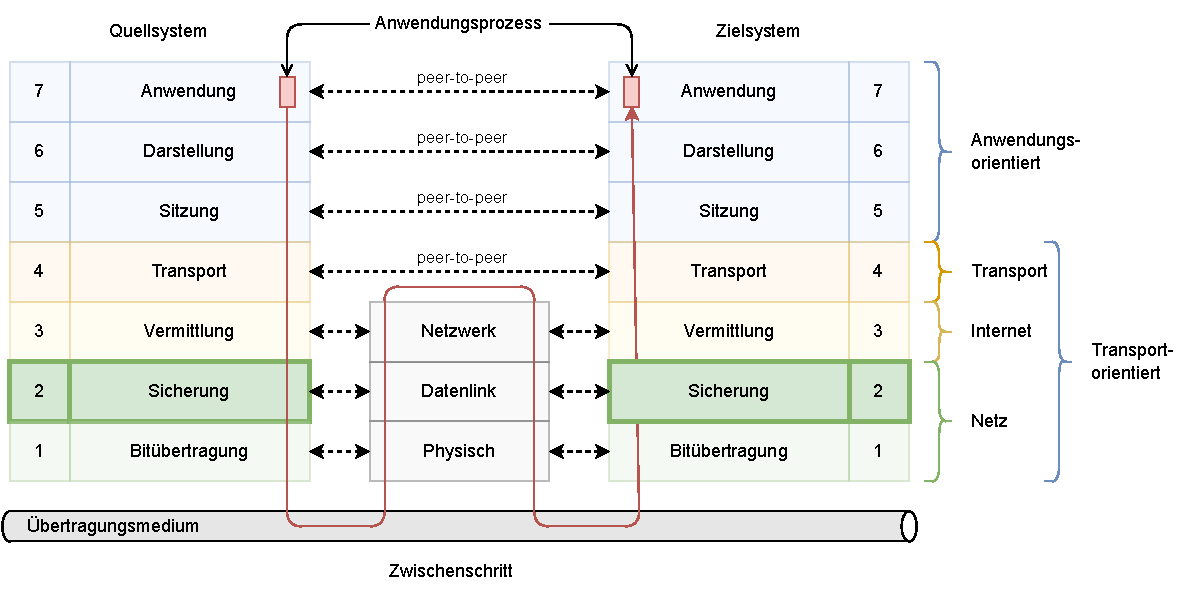
\includegraphics[width=\textwidth]{includes/figures/defi_iso_osi_sicherung.pdf}

\subsection{Übertragungsmedien}

\begin{defi}{Kupferdoppelader (Twisted Pair)}
    Bei der \emph{Doppelader} handelt es sich um eine Leitung aus zwei Einzeladern (isolierte Drähte), deren Leiterwerkstoff in der Regel aus Kupfer besteht.

    Daten werden als Spannungsniveaus übertragen und sind anfällig für Störungen\footnote{Geräte oder andere Kabel in der Umgebung, die elektromagnetische Felder ausstrahlen, verfälschen die Darstellung der Bits auf dem Kupferkabel.}.

    Die beiden Einzeladern sind entweder miteinander (\emph{Twisted Pair}) oder mit weiteren Adern verdrillt.
    Die Verdrillung sorgt dafür, dass elektromagnetische Interferenzen reduziert werden.

    Unterscheidung nach Kategorie:
    \begin{itemize}
        \item \emph{CAT 3}:
              \begin{itemize}
                  \item Gemeinsame Umhüllung für vier Kupferdoppeladern.
              \end{itemize}
        \item \emph{CAT 5}:
              \begin{itemize}
                  \item Wie CAT 3, aber mehr Windungen pro cm
              \end{itemize}
        \item \emph{CAT 6,7}:
              \begin{itemize}
                  \item Die Paare sind zusätzlich einzeln mit Silberfolie umwickelt.
              \end{itemize}
    \end{itemize}

    Unterscheidung nach Abschirmung:
    \begin{itemize}
        \item \emph{UTP Kabel} (Unshielded Twisted Pair):
              \begin{itemize}
                  \item Keine Abschirmung des Kabels
              \end{itemize}
        \item \emph{STP Kabel} (Shielded Twisted Pair):
              \begin{itemize}
                  \item Abschirmung des Kabels, dadurch günstigere Eigenschaften
              \end{itemize}
    \end{itemize}
\end{defi}

\begin{defi}{Koaxialkabel}
    \emph{Koaxialkabel} sind zweipolige Kabel mit konzentrischem Aufbau.
    Sie bestehen aus einem Innenleiter (Seele), der in konstantem Abstand von einem hohlzylindrischen Außenleiter umgeben ist.
    Der Außenleiter schirmt den Innenleiter vor Störstrahlung ab.

    Daten werden als Spannungsniveaus übertragen, sind aber im Vergleich zur Kupferdoppelader besser abgeschirmt und damit weniger störanfällig.
\end{defi}

\begin{defi}{Glasfaser}
    Eine \emph{Glasfaser} ist eine aus Glas bestehende lange dünne Faser.

    Glasfasern werden unter anderem als Lichtwellenleiter in Glasfasernetzen zur optischen Datenübertragung verwendet.
    Dies hat gegenüber elektrischer Übertragung den Vorteil einer erheblich höheren maximalen Bandbreite.

    Es können mehr Informationen pro Zeiteinheit übertragen werden, außerdem ist das übertragene Signal unempfindlich gegenüber elektrischen und magnetischen Störfeldern und in höherem Maße abhörsicher.
\end{defi}

\begin{bonus}{Dispersion}
    Für lange Glasfaserkabel gehört die (Polarisationsmoden-)\emph{Dispersion} mit zu den Faktoren, die die maximale Bandbreite der Datenübertragung begrenzen.

    Als (Polarisationsmoden-)Dispersion (PMD) wird der Effekt bezeichnet, bei dem sich Licht unterschiedlicher Polarisation verschieden schnell in einem Lichtwellenleiter ausbreitet und demnach unterschiedlich schnell vorwärts kommen.

    Des Weiteren ist die PMD abhängig von der Verlegung der Glasfaser und verändert ihren Wert, wenn Zug-, Druck- oder Torsionskräfte auf die Glasfaser ausgeübt werden.
    Ebenfalls können auch Temperaturschwankungen die Glasfaser beeinflussen.

    Aufgrund des PMD kann bei der Planung von hochbitratigen Glasfaser-Übertragungsstrecken nicht von der theoretisch möglichen Übertragungskapazität ausgegangen werden.
    Sondern es müssen sicherheitshalber Reserven berücksichtigt werden.
    Dies passiert, wenn z. B. die Glasfaser in Erdseilen von Hochspannungsstrecken verlegt werden soll.
\end{bonus}

\subsection{Netztopologien}
\label{ssec:netztopologien}

\begin{defi}{Bus}
    \begin{wrapfigure}{r}{0.25\textwidth}
        \centering
        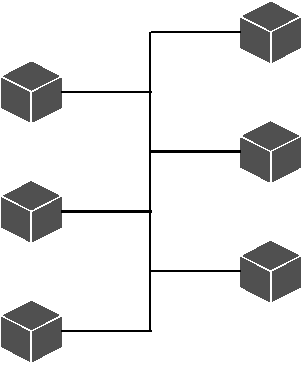
\includegraphics[width=0.2\textwidth]{includes/figures/defi_bus.pdf}
    \end{wrapfigure}%
    %
    Bei einer \emph{Bus}-Topologie sind alle Geräte direkt mit demselben Übertragungsmedium, dem Bus verbunden.
    Es gibt keine aktiven Komponenten zwischen den Geräten und dem Medium.

    Er ist einfach, preiswert und neue Knoten können einfach angeschlossen werden.
    Auch ist der Ausfall eines Knotens für die Anderen kein Problem.

    Findet eine momentane Datenübertragung zwischen zwei Teilnehmern statt, so müssen die übrigen Teilnehmer zur selben Zeit schweigen, da sie sonst stören würden.
\end{defi}

\begin{defi}{Ring}
    \begin{wrapfigure}{r}{0.25\textwidth}
        \centering
        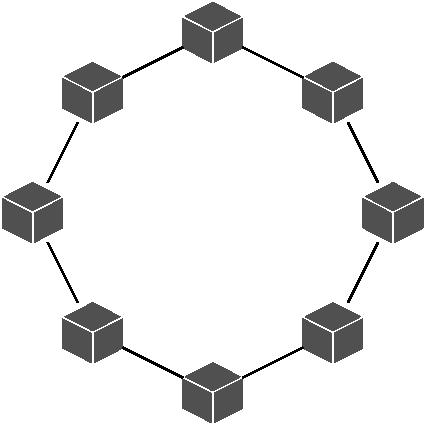
\includegraphics[width=0.2\textwidth]{includes/figures/defi_ring.pdf}
    \end{wrapfigure}%
    %
    Bei der Vernetzung in \emph{Ring}-Topologie werden jeweils zwei Teilnehmer über Zweipunktverbindungen miteinander verbunden, so dass ein geschlossener Ring entsteht.

    Die zu übertragende Information wird von Teilnehmer zu Teilnehmer weitergeleitet, bis sie ihren Bestimmungsort erreicht.
    Da jeder Teilnehmer gleichzeitig als Repeater wirken kann (wenn keine Splitter eingesetzt werden), also das Signal wieder verstärkt bzw. auffrischt, können auf diese Art große Entfernungen überbrückt werden.

    Wird im Ring nur in eine (Dreh-)Richtung kommuniziert, dann wird bei einem Ausfall von einem der Teilnehmer der Ring unterbrochen.

    In einem Ring mit Protection sind alle Leitungen doppelt; dadurch gibt es eigentlich zwei Ringe, ein \enquote{Arbeitsweg} und ein \enquote{Ersatzweg}.
    Die beiden Ringe werden meist in gegensätzlicher \enquote{Drehrichtung} betrieben.
    Wenn an einer Stelle ein oder beide Ringe unterbrochen wurden, kann immer noch jeder Teilnehmer jeden anderen erreichen.
\end{defi}

\begin{defi}{Stern}
    \begin{wrapfigure}{r}{0.25\textwidth}
        \centering
        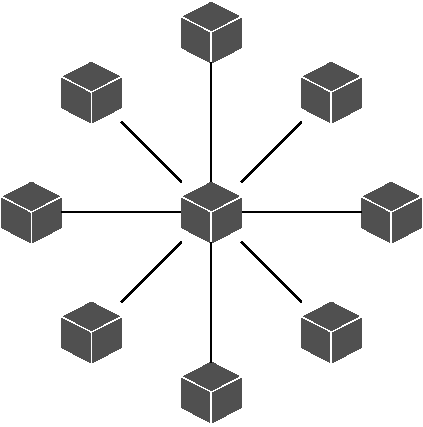
\includegraphics[width=0.2\textwidth]{includes/figures/defi_stern.pdf}
    \end{wrapfigure}%
    %
    Bei Netzen in \emph{Stern}-Topologie sind an einen zentralen Teilnehmer alle anderen Teilnehmer mit einer Punkt-zu-Punkt-Verbindung angeschlossen.
    In Computernetzen kann es eine spezialisierte Einrichtung sein, zum Beispiel ein Switch.

    In jedem Fall bewirkt eine zentrale Komponente in einem Netz eine höhere Ausfallwahrscheinlichkeit für die einzelnen Verbindungen:
    ein Ausfall des zentralen Teilnehmers bewirkt unweigerlich den Ausfall aller Verbindungsmöglichkeiten zur gleichen Zeit.
    Eine geläufige Schutzmaßnahme bei Sternnetzen besteht darin, die zentrale Komponente zu doppeln (Redundanz).
\end{defi}

\begin{defi}{Baum}
    \begin{wrapfigure}{r}{0.25\textwidth}
        \centering
        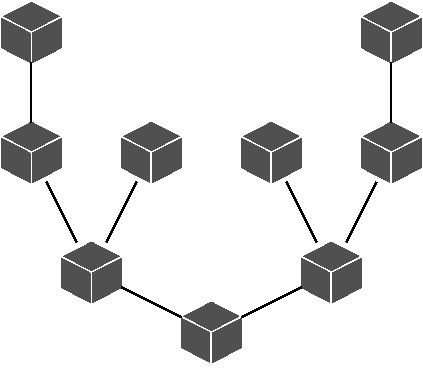
\includegraphics[width=0.2\textwidth]{includes/figures/defi_baum.pdf}
    \end{wrapfigure}%
    %
    \emph{Baumtopologien} sind dadurch gekennzeichnet, dass sie eine Wurzel (der erste bzw. obere Knoten) haben, von der eine oder mehrere Kanten (Links) ausgehen.
    Diese führen weiterhin zu einem Blatt (Endknoten) oder rekursiv zu inneren Knoten von Teilbäumen.

    Die Baum-Topologie ist nah verwandt mit der Stern-Stern-Topologie, ggf. jedoch mit strengerer hierarchischer Ordnung.

    Hierbei müssen Verbindungen zwischen den Verteilern (Hub, Switch) mittels eines Uplinks hergestellt werden.

    Häufig wird diese Topologie in großen Gebäuden eingesetzt.

    Bei Ausfall eines Verteilers (innerer Knoten) ist der ganze davon ausgehende (Unter)Baum des Verteilers nicht mehr erreichbar
\end{defi}

\subsection{Netzinfrastruktur}

\begin{defi}{Repeater}
    Ein \emph{Repeater} befindet sich in einiger Entfernung zum Sender, empfängt dessen Signale und sendet sie in aufbereiteter Form weiter, wodurch eine größere Distanz überbrückt werden kann.

    Beim Einsatz digitaler Übertragungsverfahren kann das Signal zusätzlich vom Repeater dekodiert werden, wodurch Signalstörungen (wie Rauschen oder Verzerrungen der Pulsform) entfernt werden.
    Anschließend wird das Signal wieder neu kodiert, moduliert und weitergesendet.

    In Rechnernetzen sind Repeater Bestandteile der Bitübertragungsschicht (Schicht 1 des OSI-Modells), zur Erweiterung von Netzsegmenten.

    \centering
    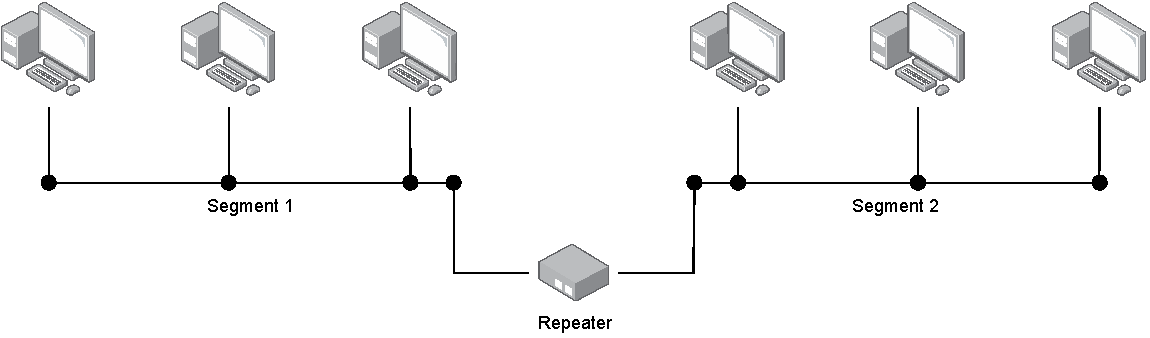
\includegraphics[width=.7\textwidth]{includes/figures/defi_repeater.pdf}
\end{defi}

\begin{defi}{Hub}
    Als \emph{Hub} werden Geräte bezeichnet, die Netzwerkknoten (physisch) sternförmig verbinden.

    Das Signal eines Netzteilnehmers wird nicht analysiert, sondern nur die übertragene Bit- bzw. Symbolebene wird regeneriert.
    Zur Kollisionserkennung trägt ein Hub allerdings meistens bei.

    Im Gegensatz zum Switch, der sich zielgerichtet Ports des Empfängers sucht, werden Bits bzw. Symbole an alle anderen Netzteilnehmer weitergeleitet (vergleiche Broadcast).

    Aus diesem Grund kann man an jedem Anschluss eines Hubs (im Gegensatz zu denen eines Switches) auch den Datenverkehr zwischen Netzwerkteilnehmern mit Netzwerksniffern analysieren oder mitschneiden.

    Ein Hub arbeitet ausschließlich auf Ebene 1 des ISO/OSI-Referenzmodells.

    \centering
    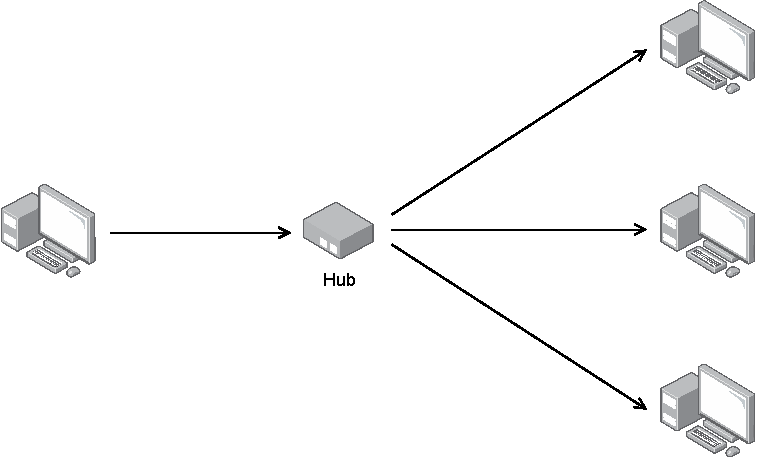
\includegraphics[width=.6\textwidth]{includes/figures/defi_hub.pdf}
\end{defi}

\begin{defi}{Switch}
    \emph{Switch}  bezeichnet ein Kopplungselement in Rechnernetzen, das Netzwerksegmente miteinander verbindet.

    Es sorgt innerhalb eines Segments (Broadcast-Domain) dafür, dass die Datenpakete (Frames) an ihr Ziel kommen.

    Im Unterschied zu einem auf den ersten Blick sehr ähnlichen Repeater-Hub werden Frames aber nicht einfach an alle anderen Ports weitergeleitet, sondern nur an den, an dem das Zielgerät angeschlossen ist – ein Switch trifft eine Weiterleitungsentscheidung anhand der selbsttätig gelernten Hardware-Adressen der angeschlossenen Geräte.

    Der Begriff Switch bezieht sich allgemein auf eine \emph{Multiport-Bridge} – ein aktives Netzwerkgerät, das Frames anhand von Informationen aus dem Data Link Layer (Layer 2) des OSI-Modells weiterleitet.

    \centering
    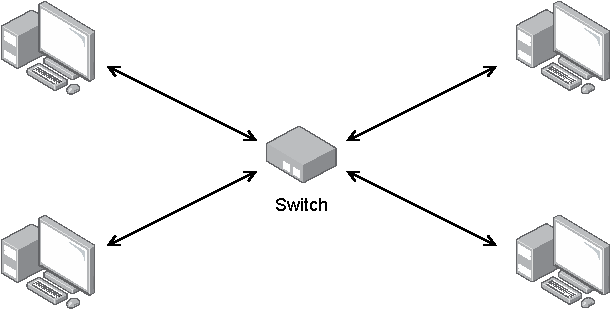
\includegraphics[width=.4\textwidth]{includes/figures/defi_switch.pdf}
\end{defi}

\begin{defi}{Bridge}
    Eine \emph{Bridge} verbindet im Computernetz zwei Segmente auf der Ebene der Schicht 2 (Sicherungsschicht) des OSI-Modells.

    Eine Bridge kann auf der Unterschicht MAC oder der Unterschicht LLC arbeiten.
    Sie wird dann \emph{MAC-Bridge} oder \emph{LLC-Bridge} genannt.

    \centering
    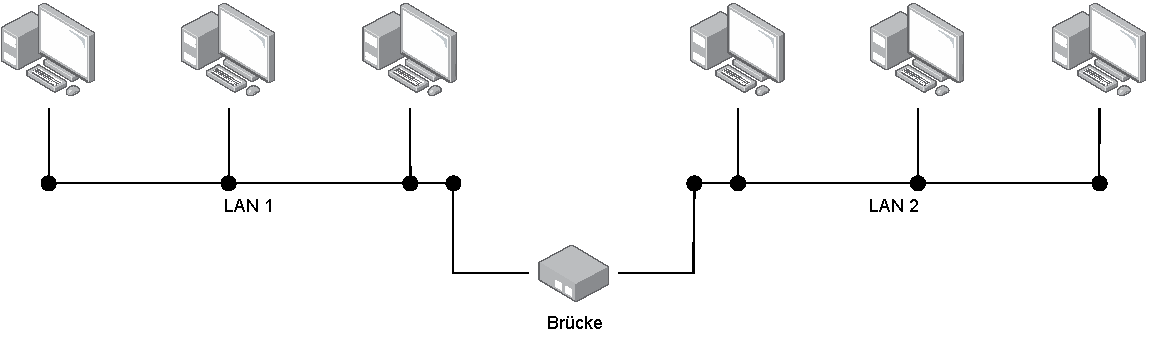
\includegraphics[width=.7\textwidth]{includes/figures/defi_bruecke.pdf}
\end{defi}

\begin{defi}{Router}
    \emph{Router} sind Netzwerkgeräte, die Netzwerkpakete zwischen mehreren Rechnernetzen weiterleiten können.
    Sie werden am häufigsten zur Internetanbindung, zur sicheren Kopplung mehrerer Standorte (Virtual Private Network) oder zur direkten Kopplung mehrerer lokaler Netzwerksegmente, gegebenenfalls mit Anpassung an unterschiedliche Netzwerktechniken (Ethernet, DSL, PPPoE, ISDN, ATM etc.) eingesetzt.

    Router treffen ihre Weiterleitungsentscheidung anhand von Informationen aus der Netzwerk-Schicht 3 (für das IP-Protokoll ist das der Netzwerkanteil in der IP-Adresse).

    Viele Router übersetzen zudem zwischen privaten und öffentlichen IP-Adressen (Network Address Translation (NAT) bzw. Port Address Translation (PAT)) oder bilden Firewall-Funktionen durch ein Regelwerk ab.

    % \centering
    % \includegraphics[width=\textwidth]{includes/figures/defi_router.pdf}
\end{defi}

\subsection{Dienste der Sicherungsschicht}

\begin{defi}{Media Access Control}
    \emph{Media Access Control} (MAC) ist eine Erweiterung des OSI-Modells.

    Dabei wird die Sicherungsschicht (Schicht 2) des OSI-Modells unterteilt in die Unterschichten \emph{Media Access Control} (2a) und \emph{Logical Link Control} (2b), wobei die MAC die untere der beiden ist.
\end{defi}

\begin{defi}{MAC-Layer}
    Die Media Access Control (MAC) ist die zweitunterste Schicht im erweiterten OSI-Modell und umfasst Netzwerkprotokolle und Bauteile, die regeln, wie sich mehrere Rechner das gemeinsam genutzte physische Übertragungsmedium teilen.

    Sie wird benötigt, weil ein gemeinsames Medium nicht gleichzeitig von mehreren Rechnern verwendet werden kann, ohne dass es zu Datenkollisionen und damit zu Kommunikationsstörungen oder Datenverlust kommt.

    Im ursprünglichen OSI-Modell war eine solche Konkurrenz um das Kommunikationsmedium nicht vorgesehen, weshalb die MAC dort nicht enthalten ist.
\end{defi}

\begin{defi}{LLC-Layer}
    \emph{Logical Link Control (LLC)} ist die Bezeichnung für ein Netzprotokoll in Schicht 2b des ISO/OSI-Modells.

    Ziel des Protokolls ist die Transparenz unterschiedlicher auf MAC-Ebene eingesetzter Verfahren zur Medienzuteilung.

    Daten, welche die OSI-Schicht 3 zur Übermittlung sendet, werden von LLC an den darunterliegenden MAC-Layer weitergegeben.
    Eingehende Daten werden von der LLC verteilt, indem sie diese an die entsprechenden Instanz-Protokolle der übergeordneten OSI-Schicht 3 weiterleitet.
\end{defi}

\begin{bonus}{Flusskontrolle}
    Auch die Sicherungsschicht past die Transmissionsraten den Fähigkeiten des Empfägers an und verhindert so etwaige Pufferüberläufe.
\end{bonus}

\begin{bonus}{Fehlererkennung}
    Fehler werden durch elektromagnetisches Rauschen und Signaldämpfung verursacht.

    Durch den Einsatz redundanter Fehlererkennungsbits kann der Empfänger Fehler erkennen (\texttt{NAK} oder Eliminieren des Frames).
\end{bonus}

\begin{bonus}{Fehlerbehebung}
    Je nach Redundanz der Fehlererkennungsbits können einige Fehler sogar ohne erneute Übertragung korrigiert werden (\emph{Forward Error Correction (FEC)}).
\end{bonus}